\documentclass[12pt,a4paper]{article}
\usepackage{listings,xcolor,setspace,hyperref,dirtree}
\usepackage{catchfile,pgffor,graphicx,float,caption}
\usepackage[margin=2.5cm]{geometry} % Set page margin to 2.5cm
\usepackage{etoolbox}
\usepackage{times} % Use Times New Roman font
\usepackage[style=numeric,backend=biber]{biblatex}

\addbibresource{paper/bibliography.bib}

\author{Florian Donnelly}
\title{The Creation of a Programming Language}

% Specify the version
\newcommand{\ver}[1]{
    \expandafter\ifstrequal\expandafter{\jobname}{paper}
    {#1}{}
}

% hyperref abbreviations
\newcommand{\hr}[2]{\hyperref[#2]{#1}}
\newcommand{\hrc}[1]{\hyperref[#1]{#1}}

% Read contents of files.txt into \files
\CatchFileDef{\files}{paper/files.txt}{\endlinechar=-1}

% Include C code from file #1 from lines #2 to #3
\newcommand{\sourcecode}[3] {
    \ver{
    \lstset{basicstyle=\scriptsize,keywordstyle=\color{blue},stepnumber=5,
        stringstyle=\color[rgb]{.3,.5,.1},commentstyle=\color{gray},
        morecomment=[l][\color{magenta}]{\#},
        postbreak=\mbox{\textcolor{red}{$\hookrightarrow$}\space}}
    \lstinputlisting[language=C,numbers=left,breaklines=true,
        frame=single,title=#1,firstnumber=#2,firstline=#2,lastline=#3]{#1}
    }
}

\newcommand{\code}[3] {
    \ver{

    \begin{minipage}{\linewidth}

    \lstset{basicstyle=\scriptsize,keywordstyle=\color{blue},stepnumber=5,
        stringstyle=\color[rgb]{.3,.5,.1},commentstyle=\color{gray},
        morecomment=[l][\color{magenta}]{\#},
        postbreak=\mbox{\textcolor{red}{$\hookrightarrow$}\space}}
    \lstinputlisting[language=C,numbers=left,breaklines=true,
        frame=single,title=\hrc{#1},
        firstnumber=#2,firstline=#2,lastline=#3]{#1}

    \end{minipage}
    }
}

% remove heading from lof
\makeatletter
\renewcommand\listoffigures{%
        \@starttoc{lof}%
}
\makeatother

% set caption width
\captionsetup{width=.7\linewidth}


% Cite text
\DeclareCiteCommand{\cte}
  {\usebibmacro{prenote}}
  {\usebibmacro{citeindex}%
   \usebibmacro{cite}}
  {\multicitedelim}
  {\usebibmacro{postnote}}

% Center text on newline
\newcommand{\expr}[1] {
    \begin{center}
        #1
    \end{center}
}

\newcommand{\paste}[1]{
    \begin{tabular}{c}
    \lstinputlisting[inputencoding=utf8,extendedchars=true,
        basicstyle=\tiny\bfseries,language={}]{#1}
    \end{tabular}
}

% the name of the programming language
\newcommand{\name}{\emph{TestScript}}
\newcommand{\pagelabel}[1]{\phantomsection\label{#1}}

% Set line spacing
\onehalfspacing




\begin{document}

\begin{titlepage}\begin{center}

    \vspace*{1.5cm}
    \Huge
    \textbf{The Creation of a Programming Language}

    \vspace{1.5cm}

    % Include Mandelbrot on title page
    \ver{
    \begin{figure}[H]
        \centering
        \paste{paper/mandelbrot.tex}
        \caption{ASCII representation of the Mandelbrot Set, generated with \name{}}
        \label{f_mandelbrot}
    \end{figure}
    }


    \Large
    \vspace{1.5cm}
    Matura Paper by\\ \textbf{Florian Donnelly}
    
    \vspace{0.5cm}
    With Supervision of\\ \textbf{Adrian Lüthi}

    \vfill
    Gymnasium Burgdorf\\ October 31, 2022

\end{center}\end{titlepage}

\normalsize

\abstract{
    This is an abstract...
}

\tableofcontents\newpage

\section{Introduction}
The importance of computers in today's world is unquestioned.
But computers are not just the metals and semiconductors they are built from,
but would be unusable without any software running on them.
Creating programs, no matter if games, web browsers or even operating systems,
involve the use of programming languages.
Those serve as a bridge between the human mind and its imagination, and
the capabilities of computer hardware and are a huge time-saver when compared
to writing machine-native code, i.e. not using a programming language.
By making use of just the term \emph{language} this paper will refer to programming
languages specifically. Sources are mentioned after cohesive paragraphs in
square brackets, an index can be found in the \emph{Bibliography} on page
\pageref{bibliography}.

Since the year 1973, when the first programming language was invented, the
research in programming languages has vastly advanced. But the goal has stayed
the same, to make programming as intuitive and easy, yet fast and efficient as
possible.

A programming language is itself only a description or specification, i.e. a
set of grammar rules defining how single instructions and entire programs
can be written. Source code, which is a program written in a certain language,
has to be understood by the computer hardware in order to run. It can either
be translated to machine-native bytecode with the help of a compiler, or
read line-by-line and interpreted by another program known as interpreter.
Such compilers or interpreters are programs on their own that are classified
as programming language implementation. The focus of this paper will be to
create such a programming language implementation, more specific an interpreter
of the custom-made \name{} language.

\subsection{Goals}
The focus of this project is learning about the internal design of interpreters
by creating a custom interpreter named \name{} interpreter, building upon
known strategies and algorithms used in existing programming languages.
The goal of this paper is to further understand the inner workings of
interpreters, stepping through human-readable source code and computing
desired results.

Modern programming languages often times provide additional tools aside from
the implementation. This includes dependency management tools to
easily create projects extending upon existing ones, or a web platforms for
people to share their code, all of which is not subject of this paper.
The \name{} implementation will also not include many features seen in modern
languages, as those are often created in years of time spent planning and
programming.

One more goal is to learn and understand the C programming language, in which
the interpreter of \name{} will be written in.

\section{Theory}
\subsection{Different Types of Interpreters}
In computing, there are several types of interpreters that behave differently.
Here are some examples and their use-cases:
\begin{itemize}
    \item \emph{Just in time Compiler.} JIT-compilers blur the line between
        classical interpreters and compilers. As the name suggests, code is
        being compiled at run time of the program. The JIT-compiler can optimize
        compilation of more-often used code and therefore adapt itself to
        behave somewhat close to optimally for a given use-case. Today, this 
        technique is often used instead of classical interpreters, as
        JIT-compilers come with only advantages. The most popular example of
        a JIT-compiler would be Google's V8 JavaScript engine used
        in NodeJS and any Chromium browsers.
    \item \emph{Bytecode Interpreter.} Such interpret the bytecode that was
        output by a bytecode compiler from a given piece of code. The bytecode
        is an intermediate representation of the program, used to speed up
        both compilation and interpretation. Such an intermediary bytecode is
        useful for ensuring platform independence or portability, as it will be
        the same across any machine, the only difference being the interpreter.
        The most popular example would be the Java Virtual Machine,
        a bytecode interpreter for java bytecode, also used by many other languages
        such as Kotlin, Scala or Groovy.
    \item \emph{Abstract Syntax Tree interpreter.} Source code can be
        transformed into an AST or parse tree by a parser. A simple example
        can be found in section \ref{simple_interpreter}
        on page \pageref{simple_interpreter}. Compared to bytecode interpreters
        there is a large time overhead when performing syntax related computation
        or visiting tree nodes recursively.
    \item \emph{Self interpreter.} These are interpreters that interpret the
        language they themselves are written in. This requires a program
        written in another language running an interpreter for the wanted
        language, in which runs another interpreted for and written in said
        language. Using a host language to initiate such system is called
        bootstrapping.

        Self-interpreters are closely related to self-hosting compilers. These
        are in turn compilers which are written in the language they compile.
        An example of a compiler written in itself is rustc, the Rust
        compiler, which was bootstrapped by the OCaml language.
\end{itemize}
This paper will implement a mixture form of an AST compiler and bytecode
interpreter. The advantage is that an AST carries along lots of information
not needed in later stages of interpretation which can be discarded. The AST
is converted to an intermediary bytecode format which only contains
necessary information about the program. Such bytecode can then be cached,
e.g. kept in memory, meaning it only has to be converted once and can be
used many times, also leading to a performance benefit.
[\cte{V8}, \cte{jvm}, \cte{rustc}]

\section{Implementation}
\subsection{Used Software}
At the heart of making any project in the C programming language
stands the C compiler. This project uses
\emph{gcc}, the GNU Compiler Collection, which, as the name suggests, also 
supports more languages than solely C. Substantiating the development process is 
\emph{GNU Make}, a general-purpose build system. It handles tasks like building
the final executable program step-by-step from the project source code and directory clean-up.
The C ecosystem is very easy to use on and fundamentally supported by 
\emph{GNU+Linux}, the operating system used to program on.
The code editor used was \emph{Microsoft Visual Studio Code}, providing great
help with built-in git integration and auto-completion features.
The tools \emph{Valgrind} and \emph{gdb}, the GNU Project Debugger were of great help
when trying to find of errors and memory leaks, see section \ref{memleaks} for details.
\emph{Git} is the project management and version tracking software used to back up and share
the project files on \emph{GitHub.com}, a Microsoft hosted git repository and
web front-end to store and collaborate on source code.

\subsection{The Art of Simplification}
When dealing with problems in general, it is helpful to map out and think about
the way of approaching the problem first. A common approach is to distill the
problem situation down to a simpler one and extending the solution to take into
account all important aspects later.

The problem to solve in this paper is concisely to make a computer understand
human written and -readable text, called source code, and follow the instructions
it proposes.
Most interpreters follow a plain scheme to go about this problem, but the
actual implementation of each of the steps can be heavily customized.
Here is the problem, broken down into three steps as commonly done in other
popular programming languages:
\begin{enumerate}\pagelabel{simple_interpreter}
    \item To create meaningful groups of characters from the input string. This
        process is known as tokenization and is done with the component called
        tokenizer or lexer. As an example, the string \emph{ab + cd} could result
        in three tokens, namely \emph{ab}, \emph{+} and \emph{cd}. In this case, space characters
        are simply ignored and could be left out, unlike in the English language where spaces are relevant. 
        This is only an example and the grouping of characters could be done 
        in any thinkable, logical way.
    \item To order the tokens into parse-tree, also called syntax-tree, as
        specified by rules. These rules are called a grammar.
        Creating an order is important, as some calculations depend on others, e.g. multiplication
        is always done before addition. An IT data structure that can accommodate
        such requirements is the binary tree. A binary tree consists of tree-nodes
        that each have a maximum of two other tree nodes as their children, and
        a tree node whose child they are, the parent node.
    \item To interpret the parse tree, traversing through it and following the
        instructions each of the tree-nodes represent. The outcome
        will be the result of the computation the program describes.
\end{enumerate}

As seen above, these components, or stages as they will be called in this paper,
each input and output data, where the output of one stage is the input of the
respective next stage.

\subsection{A Project Overview}
In the following paragraphs, the project in its entirety will be briefly
presented, giving an overview over files and correlations.

\subsubsection{File Structure}\label{FileStructure}
\begin{minipage}{\textwidth}

Here is a file tree overview of the project which will be referenced
several times in the following sections of this paper. In the depicted file tree
only source files are shown. No build files, executable files or files that
are of no further importance regarding \name are depicted.
\ver{\begin{flushleft}
    \scriptsize\setlength{\DTbaselineskip}{7pt}
    \dirtree{%
        .1 project root.
        .2 \hr{.gitignore}{.gitignore}.
        .2 \hr{README.md}{README.md}.
        .2 \hr{Makefile}{Makefile}.
        .2 \hr{mapop.gperf}{mapop.gperf}.
        .2 pseudocode.
            .3 \hr{parser.c}{pseudocode/parser.c}.
        .2 examples.
            .3 \hr{mandelbrot.nts}{examples/mandelbrot.nts}.
            .3 \hr{fibonacci.nts}{examples/fibonacci.nts}.
            .3 \hr{exec.nts}{examples/exec.nts}.
        .2 src.
            .3 \hr{main.c}{src/main.c}.
            .3 interpreter.
                .4 \hr{bytecode.c}{src/interpreter/bytecode.c}.
                .4 \hr{bytecode.h}{src/interpreter/bytecode.h}.
                .4 error.
                    .5 \hr{error.c}{src/interpreter/error/error.c}.
                    .5 \hr{error.h}{src/interpreter/error/error.h}.
                .4 \hr{interpreter.c}{src/interpreter/interpreter.c}.
                .4 \hr{interpreter.h}{src/interpreter/interpreter.h}.
                .4 libraries.
                    .5 \hr{libraries.c}{src/interpreter/libraries/libraries.c}.
                    .5 \hr{libraries.h}{src/interpreter/libraries/libraries.h}.
                    .5 stdlib.
                        .6 \hr{stdlib.c}{src/interpreter/libraries/stdlib/stdlib.c}.
                        .6 \hr{stdlib.h}{src/interpreter/libraries/stdlib/stdlib.h}.
                .4 \hr{localizer.c}{src/interpreter/localizer.c}.
                .4 \hr{localizer.h}{src/interpreter/localizer.h}.
                .4 mappings.
                    .5 \hr{operations.c}{src/interpreter/mappings/operations.c}.
                    .5 \hr{operations.h}{src/interpreter/mappings/operations.h}.
                    .5 \hr{mapop.c}{src/interpreter/mappings/mapop.c}.
                    .5 \hr{mapop.h}{src/interpreter/mappings/mapop.h}.
                .4 memory.
                    .5 \hr{hashtable.c}{src/interpreter/memory/hashtable.c}.
                    .5 \hr{hashtable.h}{src/interpreter/memory/hashtable.h}.
                    .5 \hr{array.c}{src/interpreter/memory/array.c}.
                    .5 \hr{array.h}{src/interpreter/memory/array.h}.
                    .5 \hr{stack.c}{src/interpreter/memory/stack.c}.
                    .5 \hr{stack.h}{src/interpreter/memory/stack.h}.
                .4 \hr{parser.c}{src/interpreter/parser.c}.
                .4 \hr{parser.h}{src/interpreter/parser.h}.
                .4 processing.
                    .5 \hr{implementations.c}{src/interpreter/processing/implementations.c}.
                    .5 \hr{implementations.h}{src/interpreter/processing/implementations.h}.
                .4 \hr{runtime.c}{src/interpreter/runtime.c}.
                .4 \hr{runtime.h}{src/interpreter/runtime.h}.
                .4 \hr{tokenizer.c}{src/interpreter/tokenizer.c}.
                .4 \hr{tokenizer.h}{src/interpreter/tokenizer.h}.
    }
\end{flushleft}}

\end{minipage}
\linebreak

As visible in the file tree, most of the source-code files, ending in .c,
have a corresponding header file ending in .h. This is due to the nature
of the compilation process of the C language, which is the host language
the \name{} interpreter is written in.
Each header file contains only information about functions, types or variables
available to other source or header files. The actual implementations or 
variable values are stored in the respective .c files.
% TODO:explain C compilation or link example, fix hash citation below

% TODO: say sth about README.md and expand it

The file mapop.gperf is also a source file. It is used in conjunction with the GNU gperf
tool. The tool creates a perfect hash function, which is output to the file
src/interpreter/mappings/mapop.c. The perfect hash function is used to translate
single- or multi-character symbols, such as '!=' and '+', to their respective
interpreter internal representation in constant time.
[\cte{c_compilation}, \cte{gperf}]

\subsubsection{Flowchart}

\ver{
\begin{figure}[H]
    \centering
    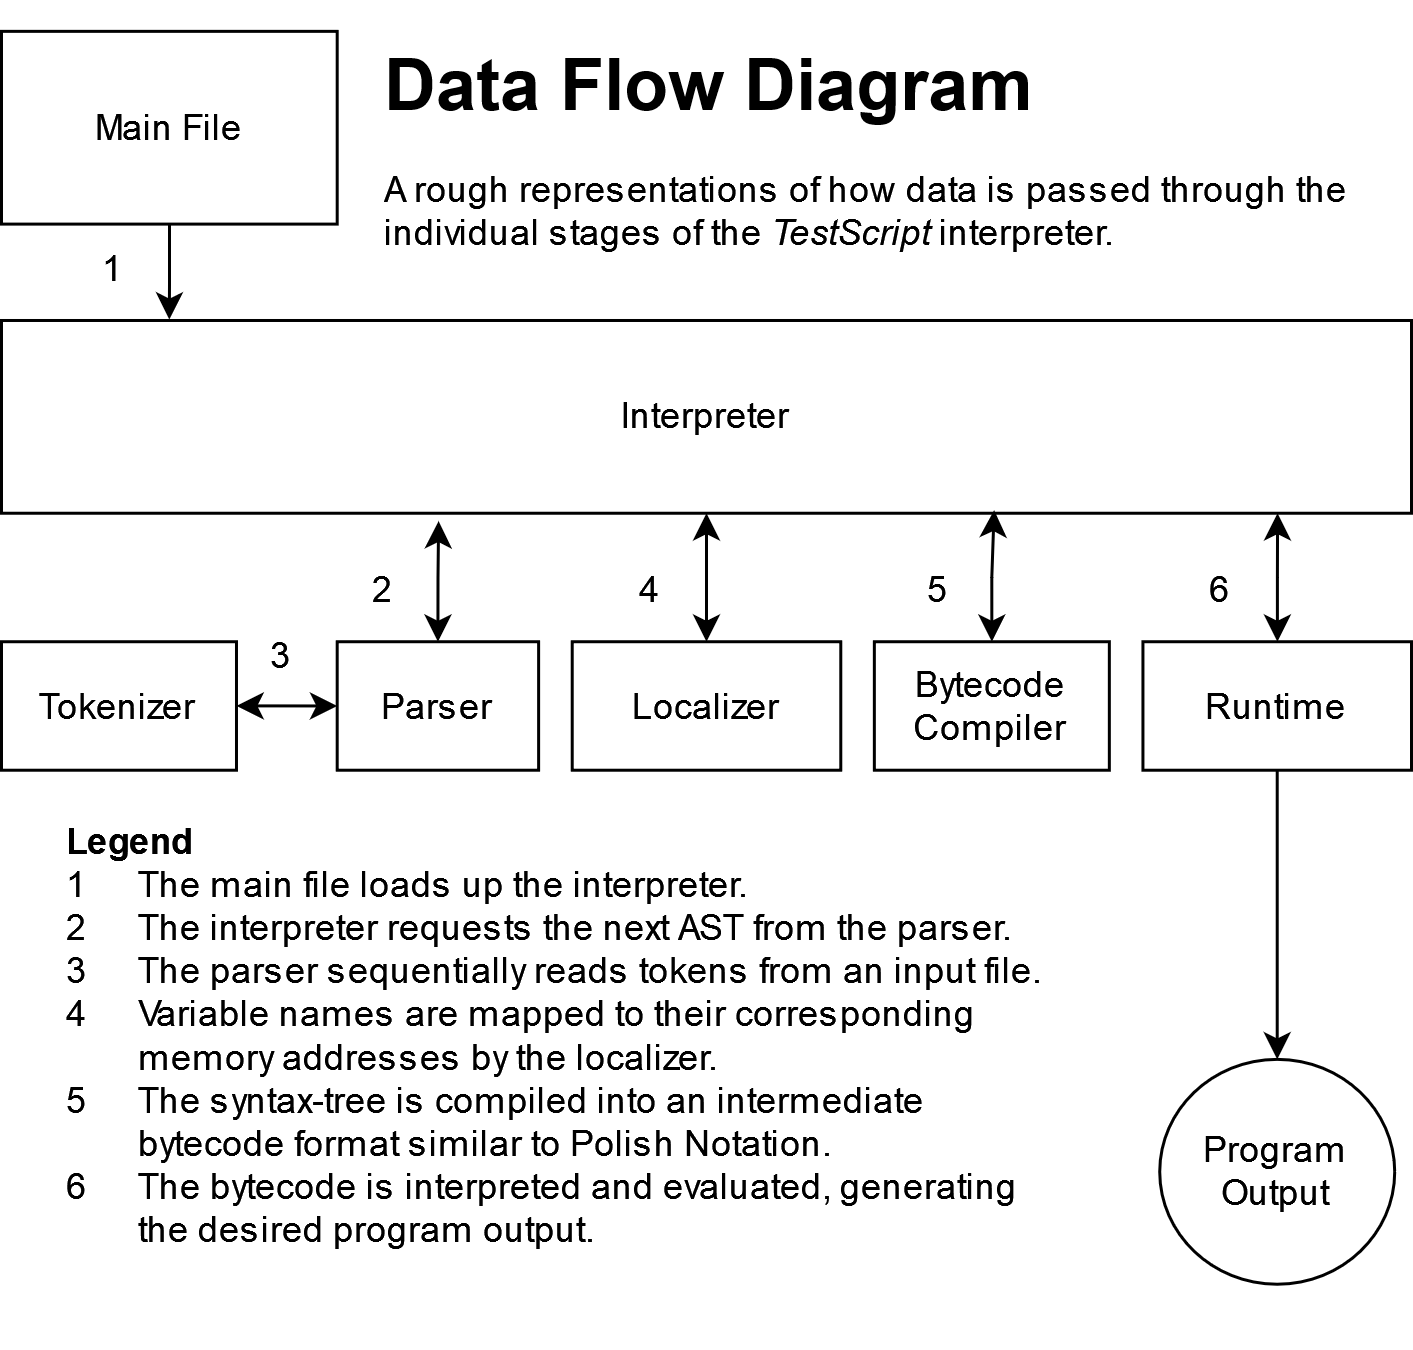
\includegraphics[width=0.6\textwidth]{paper/Data Flow Diagram.png}
    \caption{A \name{} Data Flow Diagram}
    \label{f_diagram}
\end{figure}
}

The above figure is a representation of how different components of the entire
\name{} implementation interact and work together. Each next stage performs
operations on the output data of the proper. The \hrc{src/interpreter/interpreter.c}
file, here depicted as 'Interpreter', chains all stages together.

\subsection{Implementing \name{}}
This section will explain the process of constructing and the inner workings of
the \name{} interpreter. It is therefore the most complicated and detailed section
in this paper. Examples will be made with both pseudo code and actual source
code from the project to further illustrate the decisions made during
interpreter design. The file paths used are relative to the project's root directory.

The syntax of \name{} is not specified in a formal programming language grammar,
but rather implemented from scratch in the files src/interpreter/tokenizer.c 
and src/interpreter/parser.c.

\subsubsection{The Entry-Point}
The entry point of the project lies in the \hrc{src/main.c} file.
The file implements the C main function, which is the entry-point of any
C application. Since the file is so small, here is its source code:
\code{src/main.c}{1}{999}

For the readers who do not know how to read source code, C in particular, here is a short
explanation of the basic syntax of the C language taking the \hrc{src/main.c} file
as an example:
\begin{itemize}
    \item \emph{Preprocessor Instructions.} Lines beginning with hashtags are
        C preprocessor instructions, they are dealt with by the C preprocessor.
        Preprocessing is what the compiler does before actually compiling the
        code. %TODO: add src (Preprocessor)

        The most common preprocessor instructions are the following.
        On one hand there is \expr{\#include $<$header.h$>$}
        to include various definitions from a header file, i.e. to paste
        its content at where the 'include' statement lies.
        On the other hand exists \expr{\#define A B} used to
        define A as an alias for B and replace every following occurrence of A
        with B.

    \item \emph{Functions.} In programming, functions or methods are
        a set of code that accomplish a certain task. They take in data,
        process it and return a result. Calling a function means to evaluate it for a given input.
        In C, every function has a return type, a
        function name, arguments and a function body in that order.
        Here is an example of a C function:
        \code{pseudocode/function.c}{1}{999}
        This would be an example of a main function, similar to the one
        in \hrc{src/main.c}. It returns a value
        of type \emph{int}, has two arguments, \emph{argc} and \emph{argv}, and a function body
        which, in the case of the example above, prints out the value of the \emph{argc} argument.

    \item \emph{Pointers.} Pointers are variables that store memory addresses. 
        In C syntax they can be defined with the star '*' symbol.
        An example from \hrc{src/main.c} is \expr{FILE *input;.} That means that \emph{input} is not
        actually a FILE, but rather a memory address pointing to a spot in memory where a FILE is.
        To dereference the pointer, i.e. to copy the value stored
        at the memory address into another variable, another star is used like this:
        \expr{FILE value = *input;}.
        \emph{value} now contains a copy of the actual FILE that \emph{input} was pointing to.
\end{itemize}

For those who are further interested in the C programming language, there are
countless internet articles or tutorials about reading and understanding or
writing and compiling C code. One such example is the article 'The C Beginner's
Handbook' provided by freeCodeCamp.org linked in the sources
on page \pageref{bibliography}.
[\cte{freeCodeCamp}]

Following is a very quick summary of the few 
things happening in the \hrc{src/main.c} file.
First, the \hrc{src/interpreter/interpreter.h} header file is included. 
The main function then decides whether to
read a program from a file or from standard input. 
At last, the function \emph{interpret}
from the said included header is called with the selected input.

\subsubsection{The Interpreter}
This section deals with the file 
\hrc{src/interpreter/interpreter.c} which guides
input data through the various stages of the \name{} interpreter as 
seen in figure \ref{f_diagram} on page \pageref{f_diagram}.
Following is a breakdown of the \emph{interpret} function from said file
as well as an overview of some of the stages that follow.

The function \emph{interpret} calls the parser to generate a syntax-tree from tokens retrieved
from the tokenizer implemented in \hrc{src/interpreter/parser.c} and 
\hrc{src/interpreter/tokenizer.c} respectively.

After that, the names of variables are
mapped to addresses in memory where their value is stored. Doing this before
bytecode compilation has a performance benefit. 
The mapping is achieved with a custom hash table data structure with average time
complexity of O(log n), n being the total amount of variables a \name{} program is using.
The hash table implementation used in \hrc{src/interpreter/memory/hashtable.c}                   % TODO: maybe its own paragraph! interpolation search vs binary search
uses binary search to locate elements variable-sized arrays in the hashtable's buckets.
This is because for such few variables that are used in a standard \name{} program,
an interpolation search algorithm is actually slower.
For collision detection, i.e. to circumvent problems arising when two variable names have the
same hash, a technique called separate chaining is used. In this approach, linked lists with
key-value pairs are used for each array index of the buckets and variable names are compared directly
to find exact matches.
[\cte{separate_chaining}]

The syntax tree from the parser could now be interpreted directly, but as mentioned 
before, is instead converted
to an intermediate internal bytecode format by \hrc{src/interpreter/bytecode.c}.
This step is done so that code that is run multiple times does not have
the problem of time overhead when traversing the syntax tree.

The final step is to process or execute said bytecode. This step is performed
in \hrc{src/interpreter/runtime.c}.

\subsubsection{The Tokenizer}
The tokenizer is implemented in \hrc{src/interpreter/tokenizer.c}. Its job is to
take source code in plain-text format as input and output so-called tokens.
These tokens represent groups of characters that belong together. In this paper's
implementation, each token has a strict type and a text content.
The different types of tokens and other things are defined in the header file
\hrc{src/interpreter/tokenizer.h}.

Here is an example of tokenization:
An input of \emph{a.b==23.4} would result in the following tokens according
to the tokenizer implementation of this paper:
\begin{enumerate}
    \item A token of type FIELD with content \emph{a.b}.
    \item A second token of type SYMBOL with content \emph{==}.
    \item A third token of type NUMBER with content \emph{23.4}.
\end{enumerate}
FIELD type tokens are later replaced by REFERENCE tokens, effectively mapping
variable names to addresses in memory.
SYMBOL type tokens are mapped to operators such as plus or minux by \hrc{src/implementation/mappings/mapop.c}
during parsing. NUMBER type tokens are replaced by an actual number type, which
is C's 'long double' type as specified in \hrc{src/interpreter/bytecode.h}.

While tokenizers can be programmed using regular expressions, 
this paper uses a simpler finite-state machine tokenizer.
It reads character by character, determining the token type as it goes.
It stops when there is a token that does no longer match the current token type.
Tokens are each requested and integrated into a syntax-tree by the parser as described in the next
section.

\subsubsection{The Parser}
The parser, implemented in \hrc{src/interpreter/parser.c}, generates a syntax tree,
also called parse tree, from tokens. Since this paper's implementation 
does not parse code from a
concise context free grammar, the syntax tree the parser creates is very
similar to an otherwise known abstract syntax tree, AST for short.
ASTs describe source code conceptually and do not contain all syntactical
elements required to parse code.
In this paper the terms parse tree, syntax tree and AST will be used
synonymously.

The algorithm used is inspired by the 'Pratt Parsing
algorithm' first described by Vaughan Pratt in 1973, which is a kind of precedence
parser based on recursive descent. There is an explanation of the algorithm
written by Jonathan Apodaca on \emph{dev.io} linked in the references on page 
\pageref{bibliography} which this paper's parser takes inspiration from.
[\cte{pratt}, \cte{devio}]

The syntax tree in the implementation of \name{} is a binary tree consisting of nodes, internally
called \emph{stnode}. The datatype is defined in the header file \hrc{src/interpreter/parser.h}.
Each node can either be an internal node having one or two nodes as children, or a leaf node
which stands for a value, e.g. a number or a text. Each internal node, also known as parent node, signifies
an operation done on its children. This can be an addition of two numbers for example. 

The difficult part of implementing a parser is precedence. Precedence together
with associativity define the order of execution of statements. A simple example
would be to perform multiplication before addition, e.g. \emph{2+3*4} would
result in \emph{14} and is not the same as \emph{(2+3)*4}.
Associativity is either 'Left to Right' or 'Right to Left'. An example of associativity is
\emph{20/10/2}. Both in C and in \name{}, the division operator is
left-to-right associative, meaning the stated expression is the same as
\emph{(20/10)/2} and not as \emph{20/(10/2)}. Both precedence 
and associativity are properties that are defined in the file \hrc{mapop.gpref} for
each operator.
In the end the parse tree contains all values and 
operations as well as information about the order of execution.

The parser implementation in \hrc{src/interpreter/parser.c} may be difficult to
read and understand, which is why the most important functions are explained here:
\begin{itemize}
    \item \emph{advance.} This function reads the next token from the tokenizer.
    \item \emph{secondary.} This function reads tokens that will become the leaf nodes
        of the parse tree.
        It deals with simple values that make up the start of an expression, such as numbers,
        fields, strings and it handles brackets. 
        In addition, it can handle prefix operators, such as the unary plus or unary minus.
    \item \emph{expr.} The \emph{expr} function calls \emph{secondary} whose result acts
        as the basis for a new expression. It then repeatedly checks
        if an operator follows the secondary token and creates the syntax-tree
        with help of recursive mechanisms. The nature of this function also 
        removes the need for semicolons,
        which are essential in languages like Java or C.
    \item \emph{parse.} The parse function is a small wrapper which only
        calls the \emph{expr} function a first time, initiating the parsing process.
\end{itemize}

Following is a piece of pseudo code to better illustrate the inner workings of the
parser which is based on a Pratt-parser. 
This is only an example and not completely accurate to the actual parser used
by this project.
% TODO: validate code
\code{pseudocode/parser.c}{1}{999}

\subsubsection{The Bytecode Compiler}
The bytecode compiler is an internal part of the interpreter, located in the file
\hrc{src/interpreter/bytecode.c}. Its job is to create a list
of byte-sized instructions and data from the syntax-tree the parser created.
Using such an intermediary bytecode format instead of directly interpreting
the parse-tree can be beneficial. This is the case when the same piece of code
has to be run several times. Compared to
having to walk along tree nodes recursively, reading the list of instructions in
the bytecode takes less time overall. 

Not to be confused with machine-native bytecode, the bytecode compiler in \name{}
generates byte-sequences in an internal format that are then interpreted. A
Just-In-Time compiler, JIT compiler for short, would instead compile the AST 
down to machine-native bytecode, which
runs directly on the system's hardware and does not have to be interpreted.

To generate the bytecode, \name{} recursively reads through the
binary tree created by the parser and pushes found instructions onto a stack.
The algorithm used is inspired by Edsger Dijkstra's 'Shunting yard 
algorithm', traversing the tree post-order to create
a prefix notation. 
A prefix notation is a way to write down mathematical expressions, except
operators precede their operands, in contrast to the more common infix notation,
where operands surround the operator.
[\cte{shunting_yard}]

In \hrc{src/interpreter/bytecode.c} we can see that first the left operand and then
the right operand are added onto the stack of bytecode. Therefore, when
popping from the stack and evaluating instructions, the operands will have to
be read in reverse.
Here is an example:
\begin{enumerate}
    \item Assume the following mathematical expression in infix notation:
        \expr{\emph{1 - 2 * 4 / (5 + 6)}}
    \item In common prefix notation, also called Polish notation, the
        operators would now precede the operands in this manner:
        \expr{\emph{- 1 (/ (* 2 4) (+ 5 6))}}
    \item But in \name{} the operands are pushed onto the stack is reverse order,
        as popping from the stack again reverses the order back to the original.
        This would look like the following:
        \expr{\emph{- (/ (+ 6 5) (* 4 2)) 1}}
    \item The brackets are not needed, because for every operator, the amount
        of operands is known. This is also the case for the unary minus and unary plus,
        because they are distinguished from their infix counterparts beforehand.
        The above statement would therefore look like this:
        \expr{\emph{- / + 6 5 * 4 2 1}}
        This is how expressions are represented in the bytecode of \name{}.
\end{enumerate}
[\cte{polish_notation}]

\subsubsection{Program Evaluation}
This is the last stage of interpreting program code as implemented in \name{}.
The interpreter steps through the intermediary bytecode created by the bytecode
compiler and evaluates expressions by plugging in the provided values.
All available operators are implemented in 
\hrc{src/interpreter/processing/implementations.c}.

The evaluation of expressions works in a recursive manner. Here is an 
example of \name{}'s bytecode notation and how it is evaluated:
\begin{itemize}
    \item Assume the input in \name{}'s bytecode to resemble the following expression: 
        \expr{\emph{- 6 * 3 4}}
        In common infix notation, this would be equivalent to 
        \expr{\emph{(4 * 3) - 6}.}
        The question arises, how can an algorithm compute the result of this
        calculation? The answer is recursion.
    \item The interpreter will read through the bytecode from left to right. First it will
        notice the subtraction operator and accordingly assume that two
        operands must follow.
    \item The function recursively calls itself in order to evaluate the
        right operand and notice the 6, a value and a leaf node in the parse tree. 
        The function simply returns the 6 to the subtraction expression.
    \item Again, the function calls itself to find the next operand.
        As it now reaches a multiplication operator,
        it recursively reads through that sub-expression's right and then left
        operator, which are 3 and 4 respectively.
        The result is computed and returned.
    \item Now the subtraction knows its right- and left-hand operators, 6 and 12.
        The subtraction is performed and the result, 6, is returned.
\end{itemize}

That is it. With all the operators and standard functions that have been implemented, entire programs
can be interpreted. Examples of such programs can be found in the directory
\emph{examples} of the source code.

\section{Results}

% TODO: add examples in /examples/
\name{} is built upon the implementation of a recursive Pratt
parser and a basic tokenizer. It uses a hash table to map variable names to their
memory addresses. There are no keywords, only a set of non-alphanumeric characters
representing all possible operations. Extending upon that, there are some
standard functions that enlarge the capabilities of the language.

\subsection{Syntax}
The syntax of \name{} is unlike most modern, common programming languages' syntax,
but comes closest to that of JavaScript.
In \name{}, there are no keywords at all and everything is controlled via operators,
which are non-alphanumeric characters. Such operators include the plus-sign 
for addition, the equals-sign for variable assignment or a set of brackets to signal
a function call.

Following is a piece of example \name{} code, printing out the first ten numbers
of the Fibonacci sequence, as well as a dissection of how that same code is interpreted.
\code{examples/fibonacci.nts}{1}{999}
\begin{itemize}
\item The source code begins with the definition two variables \emph{a} and \emph{b}, which
    will be utilized to keep track of the data used to calculate Fibonacci numbers.
    They are each assigned a number, zero and one respectively.
    Since the variable names \emph{a} and \emph{b} are not yet
    known to the interpreter, they are automatically allocated in the current scope
    and assigned a default value. That default value is then overwritten with the
    assignment operator.
\item Another variable \emph{count} is declared and defined as the number ten on line 4.
    This variable will be used to limit the amount of numbers the program outputs.
\item Now the function \emph{std.repeat} is called. This function is a
    standard library function, meaning it is included in the \name{} interpreter and
    written in C. Another function is passed as argument to the function call.
    This function will be repeated.
\item On line 7 and 8, some calculations are done.
    Remember, the equals sign stands for an assignment, not an
    equation. First, \emph{a} is assigned the sum of \emph{a} and \emph{b}. Then 
    \emph{b} is set to be the new \emph{a} minus \emph{b}, 
    which is in turn the same as \emph{a} before the reassignment on line 7.
\item On lines 10 and 11, the standard library function \emph{std.print} is used
    to print out the value of a and a line break. The backslash in the text
    that is print out signifies a so-called escape sequence and will be replaced with
    piece of text that can not be entered directly. The \emph{n} stands
    for a line break, but other letters such as a \emph{t} for a tabulator are possible.
\item Lastly, line 13 contains another calculation in which the variable \emph{count}
    is decremented by one. Since this is the last instruction in the inner function,
    it is simultaneously its return value, e.g. the value of count is returned
    to the \emph{std.repeat} function. The \emph{std.repeat} function will
    repeat the inner function until the returned value is zero or undefined.
    This means the inner function is executed exactly ten times, because
    the initial value of count has to be decremented by one ten times until
    it equals zero.
\end{itemize}

\subsection{Name Shadowing}
Here is another example, which in contrast to the example above, focuses on an
original security concept implemented in \name{}.
\code{examples/exec.nts}{1}{999}
The code begins by creating the variable \emph{var}, which holds a string and
\emph{f}, which calls the function \emph{std.exec} with var as argument.
Line number seven holds a comment, indicated by the two slashes at the start of the line.
Comments are ignored by the \name{} interpreter and their purpose is to contain notes
and explanations inside the source code itself. Another type of commends are block-comments
which span across multiple lines, such as on lines 9 to 12.
On line seven, the \emph{std.exec} function is called for the first time. It runs the
command it is given as argument in the user's shell, which is most commonly \emph{cmd.exe} on
Microsoft Windows and \emph{bash} on most Linux distributions. In this example, \emph{std.exec}
launches the Firefox browser, but it is capable of all kinds of things that can otherwise be
done in the shell, such as delete files or shut down the computer.

That is why in most cases, the \emph{std.exec} function can be a risk waiting to be exploited
by malicious \name{} programs. To solve this problem, there is the hashtag-operator, whose purpose
it is to delete access to a variable through the specified name. It is used on line 13 of the
example to remove access to the \emph{std.exec} function, which is why the call to that function
on line 16, trying to shut down the computer, will result in an error. Unexpectedly though, the
call on line 20 to the function \emph{f} which was created as an as to \emph{std.exec} will work.

This security concept enforces the use of a top-down programming model. First, safe to use aliases
to dangerous functions have to be created. Then, access to all those exploitable functions is
revoked. This way, running unknown code can only access data and functions that are being provided.
This contrasts the models of languages like Python. In Python, each separate source file can
make use of the \emph{import} keyword to include other files. Files imported this way do not
have access or knowledge about the variables that exist in the file that includes them.
In \name{}, each imported file would instead have access to all variables and functions that
are made available to it, instead of having to include or import them separately.
This leads to another problem, but that is what the next section will be all about.

% TODO: link more examples

\section{Discussion}
The following paragraphs will go over some positive results and some caveats of the
final product.

The name \name{} was chosen, because it implied this programming language
to be a learning project as well as a scripting language, which employ
high-level abstractions of underlying operations and interpret one line
at a time. The file name extension \emph{.nts} is used in the examples. This
file extension is not required, but was chosen as it stands for \emph{Not TypeScript}, because
the language neither enforces strict typing, nor is it Microsoft's \emph{TypeScript}.

\subsection{Distribution}
% TODO

\subsection{Limitations}\label{Limitations}
Unfortunately, there are limitations that make \name{} practically unusable for actual
professional projects. In this section, a few shortcomings of \name{} are listed
and discussed.

\subsubsection{Numbers}
Another goal that turned out not to be practical to achieve was to use just as much
memory for each variable as needed and not more. This means every variable would
have to be assigned a datatype, containing information about the size and possible values.
Taking C as a reference, the datatype \emph{char} is exactly one byte in size, and
can therefore be in exactly 2\^8 or 256 different states. But in C, information about
the datatype can be discarded at compile time, whereas in an interpreter like \name{} such
information needs to persist throughout the program's lifetime.

\subsubsection{Memory Leaks}\label{memleaks}
Memory leaks happen when a program reserves memory to store data, but
never frees up the space for use for other programs, even though the data
has long been forgotten about and will no longer be accessed.
In \name{}, memory leaks are a major problem. Even though barely noticeable in small
programs it interprets, \name{} does not have proper setups in place to free up
all used memory that is not used any longer.

Many programming languages, such as Java and Python,
make use of Garbage-Collection, a strategy to track unused allocated memory and
free it up automatically. While \name{} also tries to make use of this technique,
there are many flaws introduced while developing the interpreter that hinder 
Garbage-Collection from working correctly.

One reason for memory leaks is the nature of the
C programming language, in which the \name{} interpreter was written in. The C language and
compiler do not keep track of all possible states in which certain blocks of memory are
forgotten about and do not warn the developer. Instead, memory leaks happen and a program
uses much more system resources than required.
Modern alternatives for C such as Rust deal with the problem in a more elegant way. 
Rust has an ownership system in place,
in which any allocated memory is owned by a function. When the function
is done processing, the memory is automatically freed. Such a system
is a helpful tool for developers to create better programs without having to get
lost in the details.
Inventing new ways to make the job of developers easier is what programming
language design is all about.

A tool that is helpful to find and fix memory leaks is \emph{Valgrind}. It runs
the executable program against an input and finds the origins of not freed data.

\subsubsection{Single-Threaded}
The \name{} interpreter does not implement any multi-threading or multiprocessing.
These techniques make use of the multiple CPU cores available in modern computers
to run programs in parallel.
Any \name{} program can therefore
only contain instructions that run sequentially.
Since most languages used today allow increasing a
program's throughput using multi-threading, not having it at hand in \name{}
is a major limitation.

\subsubsection{Lack of a Development Environment}
This is probably the greatest problem of \name{} and any new prorgramming
languages in general.

Most widely used programming languages not only consist
of a language specification and a compiler or interpreter, but of many more
tools that surround them.
Such tools can include a package-manager, with which people around the world
can share code. Examples would be \emph{npm} or \emph{cargo}, 
the 'Node Package Manager' for JavaScript applications and and Rust's package 
manager respectively.
Another example of a helpful tool is a debugger, helping developers
find the cause of errors, so-called bugs, in their programs.
This includes the tool gdb, the GNU Project Debugger, that was used in this
project to find errors in the \name{} implementation.
[\cte{npm}, \cte{cargo}]

On the other hand, having to deal with countless package-managers for each
language can be annoying for developers. A solution is to build upon and
extend already existing languages and their tools with e.g. a new syntax.
This is exactly what Kotlin does. Kotlin can produce Java Virtual Machine
compatible bytecode, can be transcompiled, e.g. translated, into
JavaScript, or ECMAScript 5.1 to be more specific,
and it can be compiled to machine-native programs via LLVM. 
[\cte{kotlin_compile}]

% TODO: write about LLVM and recommend it lol6

\subsection{Interesting Ideas untouched}
Creating the ideal programming language takes a lot of planning and sketching
out. This section of the paper gives insight on interesting ideas or concepts
that are interesting and are used in other programming languages, but 
could not be implemented into \name{}.

\subsubsection{Foreign Function Interfaces}
A foreign function interface, often abbreviated as FFI,
is a mechanism by which one programming language can call functions written 
in another. This makes a language more attractive, as it can be used with
existing libraries from another language, instead of functions having to be
re-written. Enabling C function calls often allows a certain language to
directly interact with system libraries or the operating system itself.

Foreign function interfaces are available in many modern languages.
Examples are Java, Python and Rust.
Java enables users to call C, C++ and even assembly code with the Java Native
Interface, JNI for short, whereas within Python C function can
be run with the standard library \emph{ctypes}.

Foreign function interfaces are specially difficult to implement, or implement
right. Let us assume a programming language interpreter \name{} written in C that
would like to call some functions that are part of yet another C program or
library. The problem lies in the fact that at runtime, C does not know
structure of the functions to be called, say return- or argument-types, which
is by the way where the term foreign functions originates from. This is why the
\name{} developer would have to provide that information by re-declaring the
function inside \name{}, so that, with some trickery, data can be passed to and
received from the function in the correct format, preventing a segmentation
fault. The libffi C-library, which is also used by Java and
Python for this purpose, can be used to load and call such foreign functions.
[\cte{FFI}, \cte{JNI}, \cte{ctypes}, \cte{libffi}]

\subsubsection{Reflection}
Reflection, also called reflective programming, describes
the ability of a program to examine and modify its own structure and behavior 
at runtime. An example would be self-modifying code. This can easily be
achieved in assembly language, which inherently does not differentiate between
data and instructions.
Another example is Java, providing methods and classes in the java.lang.reflect
package that enable developers to examine and change properties or functions
of objects.
The easiest and simplest way to go about implementing Reflection in \name{} is
certainly to allow the interpretation of strings at runtime. That way, strings
holding program instructions can be created and modified and later executed.
[\cte{reflection}]

\subsection{Conclusion}
Creating an interpreter was a challenge. From the beginning on, the project
had to be planned and commented strictly, not to get lost in the complex web
of source code later on. The final product is a success, a working interpreter
hosting a custom programming language that can run human-readable programs.
Most parts of the source code are annotated with comments, giving interested
reader direct explanations of what is going on.
Although there are several limitations and shortcomings as stated in section \ref{Limitations}
of this paper, the details of the implementation brought about unexpected 
problems and solutions. The goal of this project to learn about 
the inner workings of an interpreter and
to get to know the C language has been acheived.


\section{Index}
This section contains a bibliography which links to all online articles
this project could profit from, and the list of figures.
The entire source code of \name{} can be found in the Appendix, section \ref{Appendix}.

\subsection{Bibliography}
\renewcommand*{\bibfont}{\normalsize}
\pagelabel{bibliography}\printbibliography[heading=none]

\subsection{List of Figures}\listoffigures
\vspace{1cm}
Figure \ref{f_mandelbrot} was generated using a \name{} program, the source code
can be found in the file \hrc{examples/mandelbrot.nts}.
Figure \ref{f_diagram} was created using an online diagram creation tool available
on \url{https://app.diagrams.net}.
[\cte{drawio}]

\section{Declaration of Authenticity}
Hereby I, Florian Donnelly, declare to have written this paper independently, 
also including the entire source code of \name{} by myself using resources 
listed under the \emph{Bibliography} section on page \pageref{bibliography}.
% TODO: check correctness of all file paths!! e.g. src/...

\newpage\section{Appendix}\label{Appendix}
The appendix contains the complete source code of \name{}.
See the file tree under \emph{File Structure} in section \ref{FileStructure}
to get an overview.

% Append all soruce files
\ver{
\foreach \f in \files{\pagelabel{\f}\sourcecode{\f}{1}{9999}}
}

\end{document}

